%*********************************************************************
\subsection{Simulation Experiment}\label{sub:bc_simulation_experiment}
%*********************************************************************

% Introductory paragraph
The application of the Bayesian calibration framework on the \gls[hyper=false]{trace} reflood model parameters against the \gls[hyper=false]{feba} experimental data is based on $6$ different statistical formulations, in the following referred to as \emph{calibration schemes}.
These schemes are distinguished by their respective assumption:
\begin{itemize}
	\item \texttt{w/ Bias, All}. The first calibration scheme assumes that the \gls[hyper=false]{trace} model is an imperfect simulator of the reflood phenomena in the the \gls[hyper=false]{feba} experiment.
		As such it considers a model bias term (as described furter below) in the calibration process. Furthermore, in this scheme, all available types of experimental data are considered.
		The data includes the clad temperature at different time points and at different axial locations (will be succinctly referred to below as the $TC$ output or data),
		the pressure drop at different time points and at different axial segments (referred to as the $DP$ output or data),
		and the collected liquid carryover at different time points (referred to as the $CO$ output or data).
		As mentioned, following the results of the previous chapter, only the most influential $8$ reflood model parameters are considered for the calibration. 
	\item \texttt{w/ Bias, TC}, \texttt{w/ Bias, DP}, and \texttt{w/ Bias, CO} are three variants of the scheme \texttt{w/ Bias, All} in which only one type of experimental data (respectively, output) is considered at a time for the calibration.
		The purpose of these schemes is to investigate the effect of using different types of data from the same experiment to constrain the model parameters prior uncertainties.
		The calibration is still conducted for the $8$ reflood model parameters and by considering the model bias term.
	\item \texttt{w/o Bias} is conducted to provide a comparison with the calibration. This scheme is similar to the scheme \texttt{w/ Bias, All};
		it uses all available types of experimental data to calibrate the $8$ reflood model parameters, except that no model bias term is included in the formulation.
		In essence, this scheme assumes that the \gls[hyper=false]{trace} model perfectly describes the reflood phenomena in the \gls[hyper=false]{feba} experiment.
	\item \texttt{w/ Bias, no dffbVIHT}. The last calibration scheme is conducted as to investigate the effect of excluding, from the calibration process, an influential parameter (\texttt{dffbVIHT}) that is later found from the scheme \texttt{w/ Bias, All} to be strongly correlated.
		Except for calibrating only the $7$ reflood model parameters, this scheme used similar assumptions as the first scheme.
\end{itemize}

The six calibration schemes above aim to update the prior uncertainties of the model parameters using the available experimental data from \gls[hyper=false]{feba} test No. 216.
The six posterior \gls[hyper=false]{pdf} formulation are then directly sampled using an ensemble \gls[hyper=false]{mcmc} sampler to obtain six different sets of posterior samples.
To avoid an excessive computational cost of having to run \gls[hyper=false]{trace} hundreds thousands of times (if not more), the \gls[hyper=false]{gp} metamodel for the \gls[hyper=false]{trace} model developed in Chapter~\ref{ch:gp_metamodel} is used to substitute \gls[hyper=false]{trace} run.

These different sets of samples are then analyzed to assess the effect of using different calibration schemes in constraining the prior uncertainties of the model parameters. 
Finally, the resulting posterior samples from different schemes are used in forward \gls[hyper=false]{uq} on the \gls[hyper=false]{trace} model of different \gls[hyper=false]{feba} tests (corresponding to different boundary conditions, namely system pressure and reflood rate).
This final exercise is aimed to assess the implication of the posterior uncertainties from different calibration schemes on (and their applicability for) the prediction under conditions different from the condition of the calibration data.

In the following, the important terms of Eq.~(\ref{eq:bc_observation_simulation_true}) will be discussed in the context of the present application on the \gls[hyper=false]{trace} model before detailing each calibration scheme.
Afterward, the \gls[hyper=false]{mcmc} sampler and simulation setting as well as a method to evaluate and compare different posterior prediction uncertainties are presented.

%-------------------------------------------------------------------------------------------
\subsubsection{Experimental Data and Observation Layout}\label{subsub:bc_observation_layout}
%-------------------------------------------------------------------------------------------

% Introductory Paragraph
The experimental data of the \gls[hyper=false]{feba} test No. $216$ used in the present calibration is based on the report provided to the participants of the \gls[hyper=false]{premium} benchmark \cite{Skorek2013}.
The data in the report, in turn, is based on the digitization of experimental curves on the original report \cite{Ihle1984} and additional review on the associated experimental uncertainties.
Therefore this were the data used by other participants of the benchmark.

% Clad Temperature
The experimental data provided for the clad temperature ($TC$) of the \gls[hyper=false]{feba} test No. $216$ consists of $33$ time points for each of the $8$ different axial locations of the thermocouples along the test section.
\marginpar{Clad temperature ($TC$) data}
Recall that by convention in the experiment, $TC1$ corresponds to the thermocouple measurement at the top of the test section ($\approx 4.1\,[m]$), while $TC8$ corresponds to the measurement at the bottom of the section ($\approx 0.3\,[m]$).

Due to the strong discontinuity of the clad temperature around the point of quenching, the model bias term cannot be modeled using stationary \gls[hyper=false]{gp} (see Section~\ref{subsub:bc_model_bias}) as it severely violates to the constant variance assumption as function of time and axial location (at the very least, before and after the quenching occurs).
To keep the simplicity from using the stationary \gls[hyper=false]{gp} formulation, the model bias term is modeled only for the part of transient before quenching occurs.
Thus the calibration is also conducted using the data prior to quenching.
This is further justified by the fact that after quenching there is much less relevant variation in the temperature transient.

Because of the different timing of quenching along the test section, the number of data points available for calibration changes per axial location.
Based on these data points, an observation layout for $TC$ data can be defined,
\begin{equation}
	\begin{split}
		\boldsymbol{\Lambda}_{TC} & = \{(z_1,t_1),(z_1,t_{2}),(z_2,t_1),\ldots,(z_2,t_{7}),\\
															& \quad\quad (z_3,t_1),\ldots,(z_3,t_{12}),(z_4,t_1),\ldots,(z_4,t_{17}),  \\
															& \quad\quad (z_5,t_1),\ldots,(z_5,t_{21}),(z_6,t_1),\ldots,(z_6,t_{24}),  \\
															& \quad\quad (z_7,t_1),\ldots,(z_7,t_{25}),(z_8,t_1),\ldots,(z_8,t_{27})\} \\
	\end{split}
\label{eq:bc_observation_layout_feba_tc}
\end{equation}
where $z$ denotes the axial location (or segment for the $DP$ data) and $t$ denotes time point.

% Clad Temperature uncertainty

% Pressure Drop
The experimental data provided for the pressure drop ($DP$) of the \gls[hyper=false]{feba} test No. $216$ consists of $18$ time points for each of the $4$ different axial segments of the pressure drop measurements.
\marginpar{Pressure drop ($DP$) data}
Recall that in the experiment, the \emph{bottom} segment corresponds to the segment $0.0 - 1.7\,[m]$, the \emph{middle} to $1.7 - 2.3\,[m]$, the \emph{top} to $z = 2.3 - 4.1\,[m]$, and the \emph{total} to $0.0 - 4.1\,[m]$.
In the following, the bottom, the middle, the top, and the total segments are simply indices of the $DP$ output; $z_1$, $z_2$, $z_3$, $z_4$, respectively.
The observation layout for the $DP$ data is then defined as follow,
\begin{equation}
		\boldsymbol{\Lambda}_{DP} = \{(z_1,t_1),\ldots,(z_1,t_{18}),(z_2,t_1),\ldots,(z_4,t_{18})\}
\label{eq:bc_observation_layout_feba_dp}
\end{equation}
where $z$ denotes the axial location (or segment for the $DP$ data) and $t$ denotes time point.

% Pressure drop uncertainty

% Liquid carryover
Finally, the experimental data provided for the liquid carryover ($CO$) of the \gls[hyper=false]{feba} test No. $216$ initially consists of $16$ time points.
\marginpar{Liquid carryover ($CO$) data}
However, because the collecting tank was saturated at $10\,[kg]$ only the transient up to that mass is of interest.
By excluding the data points where the tank has been saturated, only $7$ data points are available for the calibration.
Based on these data points, the observation layout for the $CO$ data is defined as,
\begin{equation}
		\boldsymbol{\Lambda}_{CO}  = \{(t_1),\ldots,(t_{7})\}
\label{eq:bc_observation_layout_feba_co}
\end{equation}
where $z$ denotes the axial location (or segment for the $DP$ data) and $t$ denotes time point.

% Liquid carryover uncertainty

% Full observation layout
Finally, the observation layout for each output (data) type can be combined into a single long vector of the full observation layout,
\marginpar{Full observation layout}
\begin{equation}
	\begin{split}
		\boldsymbol{\Lambda} & = \{(TC, z_1,t_1),\ldots,(TC,z_8,t_{27}),\\
		                     & \quad\quad (DP,z_1,t_{1}),\ldots,(DP,z_4,t_{18}),\\
												 & \quad\quad (CO,t_1),\ldots,(CO,t_7)\}\\
	\end{split}
\label{eq:bc_observation_layout_feba_full}
\end{equation}
That is, by convention here, $\boldsymbol{\Lambda} = \{\boldsymbol{\Lambda}_{TC}, \boldsymbol{\Lambda}_{DP}, \boldsymbol{\Lambda}_{CO}\}$.
The total number of data points of \gls[hyper=false]{feba} test No. $216$, and the length of the observation layout $\boldsymbol{\Lambda}$, used in the calibration is thus $212$.

%--------------------------------------------------------------------------------------------
\subsubsection{Gaussian Process Approximation for TRACE Simulation}\label{subsub:bc_gp_trace}
%--------------------------------------------------------------------------------------------

%-----------------------------------------------------------------------
\subsubsection{Modeling the Model Bias Term}\label{subsub:bc_model_bias}
%-----------------------------------------------------------------------

%-----------------------------------------------------------------------
\subsubsection{Calibration Schemes}\label{subsub:bc_calibration schemes}
%-----------------------------------------------------------------------

% Summary
Table~\ref{tab:ch5_calibration_schemes} summarizes the different calibration schemes considered in this study.
\begin{table*}[!htbp]\centering
\ra{0.9}
\begin{adjustwidth*}{}{-3cm}
\caption{Bayesian calibration schemes conducted for the \gls[hyper=false]{trace} reflood model parameters against data from \gls[hyper=false]{feba} test No. $216$.}
\label{tab:ch5_calibration_schemes}
\begin{tabular}{@{}clccccrc@{}}\toprule
\multirow{2}{*}{No.} & \multirow{2}{*}{\shortstack[c]{Calibration Scheme}} 	& \multirow{2}{*}{\shortstack[c]{Model Bias\\Term}}	& \multicolumn{3}{c}{Types of Output} & \phantom{a} & \multirow{2}{*}{\shortstack[c]{Reflood Model\\Parameters \footnotesize{(total number)}}} \\
																															  \cmidrule{4-6}
    &                                 					& 						& $TC$				& $DP$     		& $CO$   				&&	\\ \midrule
1   & \texttt{w/ Bias, All}											& \Checkmark  & \Checkmark  & \Checkmark  & \Checkmark  	&& All \footnotesize{($8$)}          				\\
2   & \texttt{w/ Bias, TC}     									& \Checkmark  & \Checkmark	&							&          			&& All \footnotesize{($8$)}           			\\
3   & \texttt{w/ Bias, DP}     									& \Checkmark 	&         		& \Checkmark	&								&& All \footnotesize{($8$)} 								\\
4   & \texttt{w/ Bias, CO}       								& \Checkmark 	& 						& 						& \Checkmark		&& All \footnotesize{($8$)}           			\\
5   & \texttt{w/o Bias}               					&          		& \Checkmark  & \Checkmark  & \Checkmark		&& All \footnotesize{($8$)}	          			\\
6   & \texttt{w/ Bias, no dffbVIHT}             & \Checkmark  & \Checkmark  & \Checkmark  & \Checkmark		&& Excluding \texttt{dffbVIHT} \footnotesize{(7)}\\
\bottomrule
\end{tabular}
\end{adjustwidth*}
\end{table*}

%---------------------------------------------------------------------------------------
\subsubsection{MCMC Simulation using Ensemble Sampler}\label{subsub:bc_calibration_mcmc}
%---------------------------------------------------------------------------------------

%-----------------------------------------------------------------------------------------
\subsubsection{Evaluating Calibration Results}\label{subsub:bc_calibration_evaluation}
%-----------------------------------------------------------------------------------------


% The statistical calibration framework revisited

% Observation Layout

% Modeling the simulator output

% Modeling the discrepancy

% Likelihood Formulation

% 

% 

% 

% Analyzing convergence
\clearpage
\begin{sidewaysfigure}
	\centering
	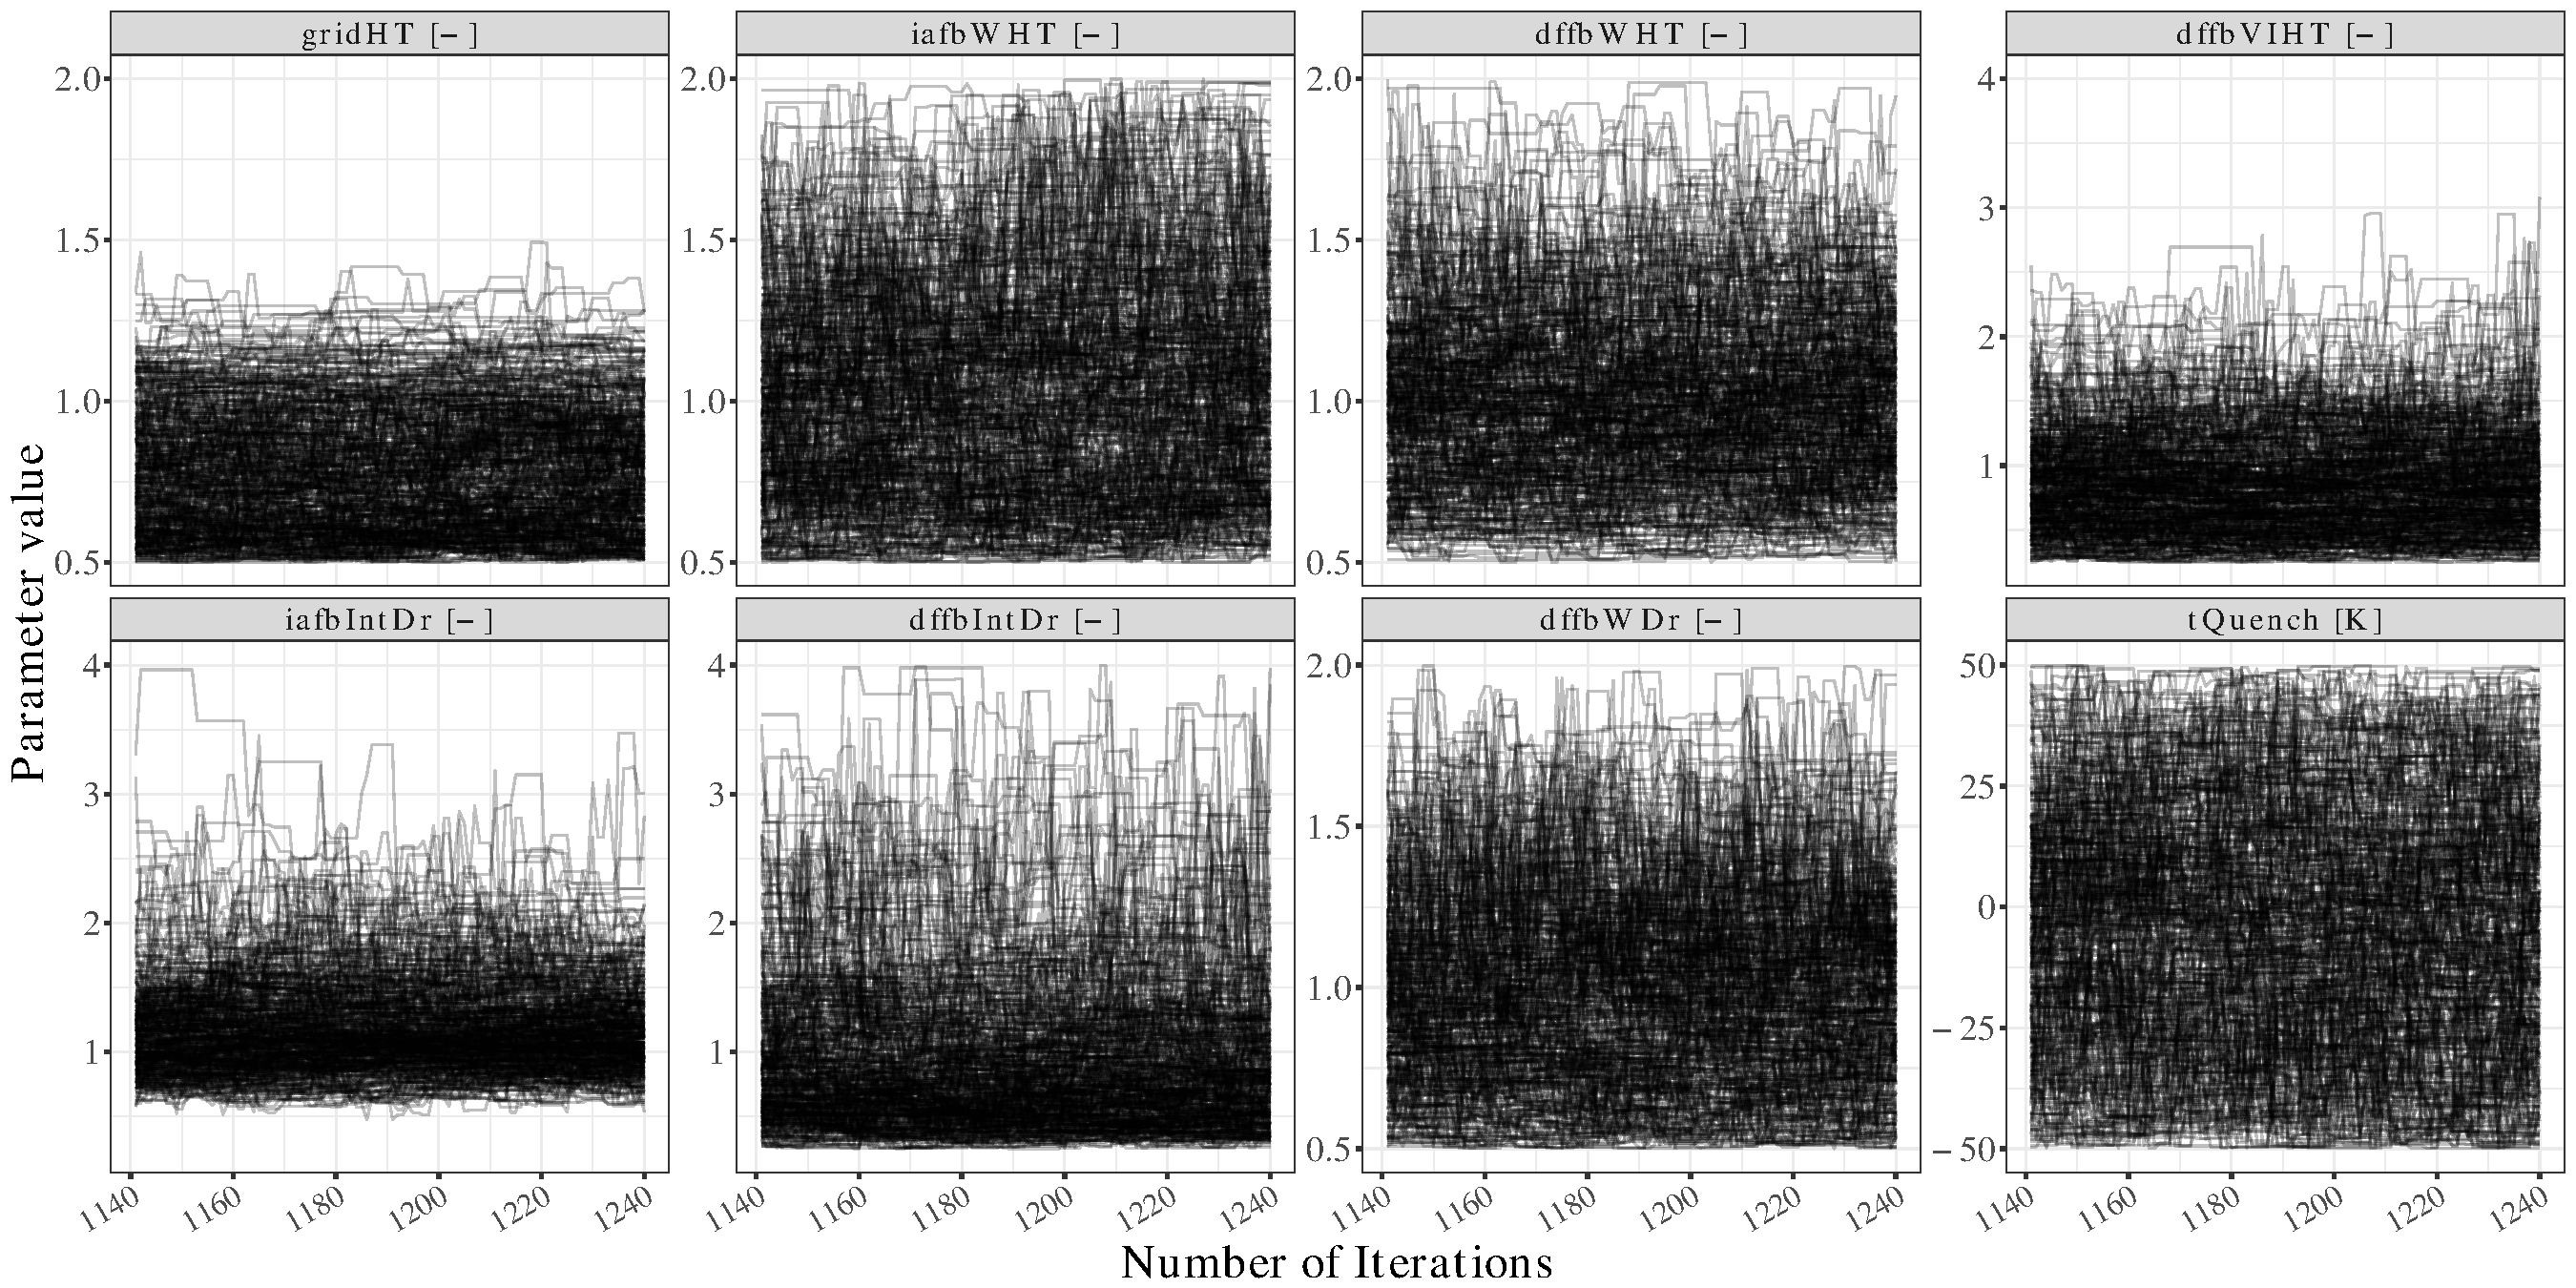
\includegraphics[width=0.90\textwidth]{../figures/chapter5/figures/plotEnsTraceDiscAllCentered}
		\captionof{figure}[Ensemble trace plots for each model parameter of calibration with model bias term.]{Ensemble trace plots for each model parameter of calibration with model bias term. Shown here is for the last $100$ iterations (out of $1'240$ post-burn-in iterations) and for $400$ walkers (out of $1'000$ walkers).}
	\label{fig:ch5_plot_ens_trace_all_disc_centered}
\end{sidewaysfigure}
\clearpage